In this section, after discussing the assumptions and system model, the problem of joint SFC deployment and VNFM placement is stated and clarified by an illustrative example.

\subsection{Assumptions}\label{subsec:assumptions}
In the JSD-MP problem, a set of SFCs need to be deployed in the physical infrastructure network.
The main assumption is that in addition to computational and network resources,
a VNFM should be assigned for each SFC to manage the VNFs of the SFC.
All VNFs of a chain should be managed by a single VNFM, but a VNFM can manage multiple SFCs.
The capacity of each VNFM is limited in terms of the number of VNF instances.
Each VNFM needs a license for managing the specific number of VNF instances.
Moreover, we assume that only a subset of physical servers can host VNFMs and similarly,
each VNF type can only be placed on a subset of physical servers. It is assumed that traffic ingress and egress of each chain are conducted by a special type of NFVs, which need to be placed on ingress and egress nodes  of the physical network respectively.

VNF instances deployed on a physical server can only be managed by the VNFMs placed on a given subset of physical servers. To maintain the timing requirement of the management traffic, the distance (in term of hop-count) between each VNFM and its associated VNFs should be less than the specified threshold.
Also, JSD-MP considers VNFs can't shared between chains.
% Only a subset of VNF types need to managed and other can be deployed without an assigned VNFM.

\subsection{System Model}\label{subsec:sysmodel}
% parameters will define here and decision variables will defined in formulation section.
%
%% Infrastructure's parameters have superscript "p"
%% Chain's parameters have superscript "s"
%% Infrastructure's nodes have subscript "i", "j"
%% Chain's nodes have subscript "u", "v"
%% Use parentheses for functions and in rare occasions
%% Management's parameters have superscript "m"
%% Use capital letters for sets
%

The physical infrastructure topology is modeled as a directed graph \(G^p=(V^p, E^p)\),
where \(V^p\) is the set of NFVI-PoPs and \(E^p\) is a set of the inter-PoP links.
The computational capacity of PoP \(i \in V^p\) is specified by \(c^p_i\) number of CPU cores and \(m^p_i\) gigabytes of RAM.
Bandwidth of link \((i,j) \in E^p\) is specified by \(b^p_{(i.j)}\).

The set of requested SFCs is denoted by \(R\).
Each request \(r \in R\) has revenue \(c_r\) and
is represented by directed graph \(G^s_r = (V^s_r, E^s_r)\),
where \(V^s_r\) is the set of VNFs and \(E^s_r\) is the set of the virtual links of the chain.
The type of VNF \(v \in V^s_r\) is denoted by \(t_{v,r} \in T\) where \(T\) is the set of the types of the functions.
Each type \(t\) determines the required number of CPU cores \(c^s_t\)
and the required amount of memory \(m^s_t\) to create an instance of that type.
The required bandwidth of each virtual link \((u,v) \in E^s_r\) is denoted by \(b^s_{(u,v),r}\).

Each VNFM requires \(c^m\) number of CPU cores and \(m^m\) gigabytes of RAM to handle \(\kappa\) number of VNFs at most. To lunching a VNFM, the service provider has to pay the license fee \(\phi\).
There is a dedicated virtual management link with bandwidth \(b^m\) between every VNF instance and its associated VNFM.
The restrictions of the placement of VNFMs and VNFs, discussed in the previous section, are formulated by a few given parameters.
We use \(\rho\) to indicate the maximum hop counts for each virtual management link. Parameter \(\eta_{(i, j)}\) indicates whether the VNFM mapped to the physical server \(i \in V^p\) can manage the VNFs placed on the physical node \(j \in V^p\) or not. 
% Parameter \(\omega_r\) indicates that type \(r \in T\) requires manager or not.
% The binary parameter \(\psi_i\) indicates that physical server \(i \in V^p\) support VNFs or not.
The notations discussed here are summarized in Table \ref{tbl:parameters}.

\begin{table}
    \caption{Parameters}
    \label{tbl:parameters}
    \begin{small}
    \begin{center}\begin{tabular}{|c|p{0.75\textwidth}|}
    \hline
    \(V^p\) & the set of NFVI-PoPs \\
    \hline
    \(E^p\) & the set of the inter-PoP links \\
    \hline
    \(c^p_i\) & number of CPU cores of server \(i\) \\
    \hline
    \(m^p_i\) & amount of RAM in server \(i\) \\
    \hline
    \(b^p_(i,j)\) & bandwidth of link \((i, j) \in E^p \) \\
    \hline
    \(V^s_r\) & the set of VNFs for the request \(r\) \\
    \hline
    \(E^s_r\) & the set of virtual links of the request \(r\) \\
    \hline
    \(m^s_t\) & required RAM of VNF instance with type \(t \in T\) in GB \\
    \hline
    \(c^s_t\) & required CPU cores of VNF instance with type \(t \in T\) \\
    \hline
    \(m^m\) & required RAM of VNFM in GB \\
    \hline
    \(c^m\) & required CPU cores of VNFM \\
    \hline
    \(\kappa\) & maximum number of VNF instances that a VNFM can handle \\
    \hline
    \(\tau(v, t)\) & function that returns 1 if the VNF instance \(v\) has type \(t\)  \\
    \hline
    \(b^s_{(u, v),r}\) & required bandwidth for virtual link \((u, v) \in E^s_r\) \\
    \hline
    \(b^m\) & required bandwidth for each virtual management link \\
    \hline
    \(\rho\) & maximum hop count of management links \\
    \hline
    \(\phi\) & VNFM license fee \\
    \hline
    \(\eta_{(i, j)}\) & binary parameter that is 1 if VNFs on physical server \(i\) can manage by VNFMs on physical server \(j\) \\
    \hline
    \end{tabular}\end{center}
    \end{small}
\end{table}

\subsection{Problem Statement}
Under the assumptions of subsection \ref{subsec:assumptions}, the JSD-MP problem is defined as following using the notations defined in subsection \ref{subsec:sysmodel}.
The NFVI service provider owns the infrastructure network \(G^p\). A set \(R\) of requests are given. The service provider's goal is to accept a subset of requests that maximize the profit.
To accept a request \(r\), the service provider should allocate the \(c^s_{t_{v,r}}\) CPU cores, and \(m^s_{t_{v,r}}\) amount of memory for all \(v \in r\);
moreover, \(b^s_{(u,v),r}\) bandwidth should be allocated for all links \((u,v) \in E^s_r\), and a VNFM needs to be assigned for the chain.
These allocations should satisfy the requirements mentioned in subsection \ref{subsec:assumptions}.
The profit is made by the revenue obtained from accepting the requests while the service provider should pay the license cost of \(\phi\) for each VNFM.

The idea behind the JSD-MP problem is that in the placement of VNFM for a chain, the location of the VNFs of the chain should be taken into account. Therefore, by jointly conducting of SFC deployment and VNFM placement, the service provider can maximize the profit.

This problem is clarified by an illustrative example in the following subsection.

\subsection{Illustrative Example}
In this section, an illustrative example is presented to gain more sight into the JSD-MP problem.
Figure~\ref{fig:example-chains} shows two request chains where the type of VNFs and the required bandwidth of the virtual links in Mbps are depicted. Each of these requests worth 100\$.
The NFVI service provider owns the infrastructure that is shown in Figure~\ref{fig:example-topology}.
VNF's types are described in Table~\ref{tbl:example-vnf-types}, and 
Table~\ref{tbl:example-server-spec} shows the physical servers specifications.
There a few constraints on placing the VNFs and capacity of the NFVI as following.
Instances can only run on servers 1, 3, 5, and 7 since the remaining servers are fully utilized.
The VNFs on servers 1 and 3 can only be managed by the VNFMs on servers 2 and 4.
The VNFs on server 5 can only be managed by the VNFMs on servers 4 and 6.
The VNFs on server 7 can only be managed by the VNFMs on servers 6 and 8.
Each VNFM can handles at most 5 instances with 4 GB of RAM and 2 CPU cores and license that costs 10\$.
Management links requires 10Mbps reservation and maximum hop counts for management is 10.
All physical links has 40Gbps capacity. 

\begin{figure}
    \centering
    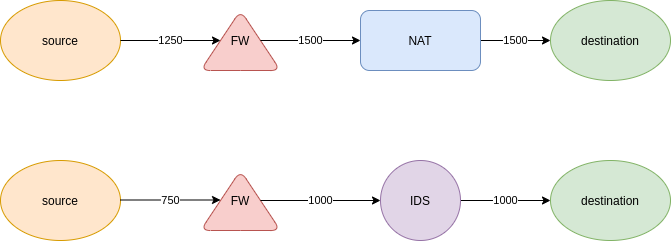
\includegraphics[width=0.7\linewidth]{images/example-chains.png}
    \caption{Chains for illustrative example}
    \label{fig:example-chains}
\end{figure}

\begin{figure}
    \centering
    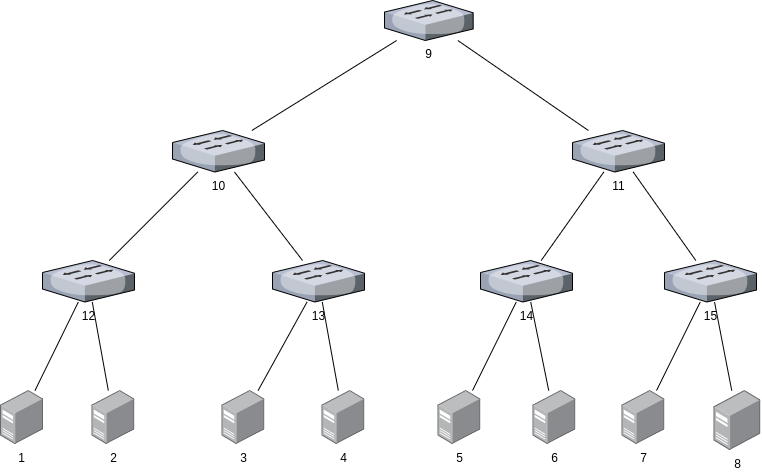
\includegraphics[height=150pt]{images/example-toplogy.png}
    \caption{Topology of illustrative example}
    \label{fig:example-topology}
\end{figure}

\begin{table}
    \centering
    \caption{VNFs type of illustrative example}
    \begin{tabular}{|c|c|c|c|}
        \hline
        Spec/VNF & vFW & vNAT & vIDS \\
        \hline
        CPU (vCore) & 2 & 2 & 2 \\
        \hline
        Memory (GB) & 2 & 4 & 2 \\
        \hline
    \end{tabular}
    \label{tbl:example-vnf-types}
\end{table}

\begin{table}
    \centering
    \caption{Server specification of illustrative example}
    \begin{tabular}{|c|c|c|}
        \hline
        & Server 1,2,7,8 & Servers 3,4,5,6 \\
        \hline
        Installed vCPU & 144 & 72 \\
        \hline
        Installed Memory (GB) & 1408 & 288 \\
        \hline
        Link (Gbps) & 40 & 40 \\
        \hline
    \end{tabular}
    \label{tbl:example-server-spec}
\end{table}

The optimal solution of this instance of the JSD-MP, which is obtained by the MILP formulation presented in section~\ref{sec:formulation}, is as following:

Two chains are accepted with using two VNFM instances that cost 20 so the total revenue is 180.
Instance mappings are shown in \ref{tbl:example-chain-1-mapping} and \ref{tbl:example-chain-2-mapping}.
Also link mappings are shown in \ref{tbl:example-chain-1-links}.

\begin{table}
    \centering
    \caption{Chain-1 Instance Mapping of illustrative example}
    \begin{tabular}{|c|c|c|c|c|}
        \hline
        0: Source & 1: FW & 2: NAT & 3: Destination & VNFM \\
        \hline
        9 & 1 & 3 & 9 & 4 \\
        \hline
    \end{tabular}
    \label{tbl:example-chain-1-mapping}
\end{table}

\begin{table}
    \centering
    \caption{Chain-1 Instance Mapping of illustrative example}
    \begin{tabular}{|c|c|c|c|c|}
        \hline
        0: Source & 1: FW & 2: IDS & 3: Destination & VNFM \\
        \hline
        9 & 3 & 3 & 9 & 4 \\
        \hline
    \end{tabular}
    \label{tbl:example-chain-2-mapping}
\end{table}

\begin{table}
    \centering
    \caption{Chain-1 Link Mapping of illustrative example}
    \begin{tabular}{|c|l|}
        \hline
        Virtual Link & Physical Links \\
        \hline
        (0, 1) & (9, 10) (10, 12) (12, 1) \\
        \hline
        (1, 2) & (1, 12) (12, 10) (10, 13) (13, 3) \\
        \hline
        (2, 3) & (3, 13) (13, 10) (10, 9) \\
        \hline
        VNF 0 Mgmt. & (9, 10) (10, 13) (13, 4) \\
        \hline
        VNF 1 Mgmt. & (1, 12) (12, 10) (10, 13) (13, 4) \\
        \hline
        VNF 2 Mgmt. & (3, 13) (13, 4) \\
        \hline
        VNF 3 Mgmt. & (9, 10) (10, 13) (13, 4) \\
        \hline
    \end{tabular}
    \label{tbl:example-chain-1-links}
\end{table}

\begin{table}
    \centering
    \caption{Chain-2 Link Mapping of illustrative example}
    \begin{tabular}{|c|l|}
        \hline
        Virtual Link & Physical Links \\
        \hline
        (0, 1) & (9, 10) (10, 13) (13, 4) \\
        \hline
        (1, 2) & --- \\
        \hline
        (2, 3) & (3, 13) (13, 10) (10, 9) \\
        \hline
        VNF 0 Mgmt. & (3, 13) (13, 10) (13, 4) \\
        \hline
        VNF 1 Mgmt. & (3, 13) (13, 4) \\
        \hline
        VNF 2 Mgmt. & (3, 13) (13, 4) \\
        \hline
        VNF 3 Mgmt. & (9, 10) (10, 13) (13, 4) \\
        \hline
    \end{tabular}
    \label{tbl:example-chain-2-links}
\end{table}
